The system implementation is divided into four main modules, Feature extraction, Pose estimation, Non-linear optimization and 3D visualization.


\begin{figure}[htb]
	\centering
	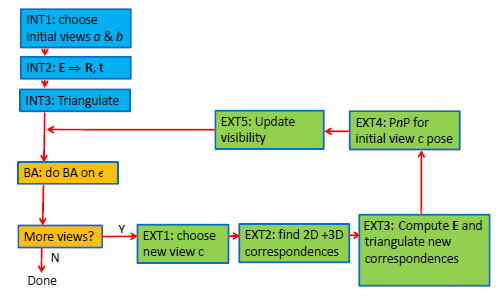
\includegraphics[width=\linewidth]{images/data_flow.png}
	\caption{\textit{Data flow between modules.}}
	\label{fig:block_overview_fig}  %Skapar referens till figuren
\end{figure}

\begin{figure}[htb]
	\centering
	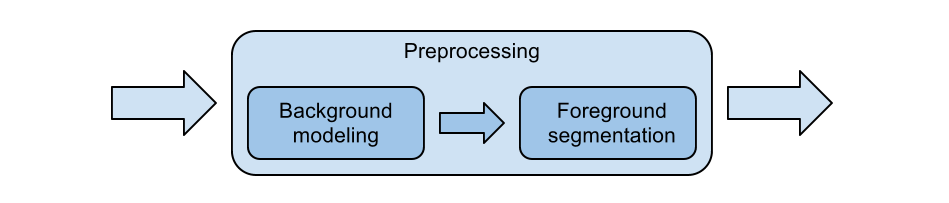
\includegraphics[width=\linewidth]{images/data_flow_preprocessing.png}
	\caption{\textit{Data flow within preprocessing block.}}
	\label{fig:block_overview2_fig}  %Skapar referens till figuren
\end{figure}


First the background model adapts to the new image and estimate which pixels belong to the background and which that do not. Multiple hypothesis of what the background actually looks like are kept using a mixture of Gaussians model.

After the background model has been updated, the foreground processing module is called upon to perform some noise removal and to detect all the interesting regions in the image (the regions considered to be foreground by the background model)

Once all the interesting regions are localized, the identification module takes all the created objects in the current frame and associates them with the proper ID. This is done by comparison with the objects in the previous frame.

To help in the labelling process we use a Kalman predictor, that predicts the position of the each object in the next frame. The Prediction module is called upon after the identification is done.